\section{Studying the presence of diabetes}

\frame{%
    \frametitle{Why diabetes?}

    \begin{itemize}
        \pause\item Of interest to the health board
        \pause\item Discussed widely in literature
        \pause\item Acts as an example for looking at condition-based slices
    \end{itemize}
}

\subsection{Distributions of key attributes and demographic information}

\frame{\frametitle{Number of spells associated with a patient}
    \makebox[\linewidth]{%
        \includegraphics[width=\imgwidth]{no_spells_bar/main.pdf}
    }
}

\frame{\frametitle{Length of stay}
    \makebox[\linewidth]{%
        \includegraphics[width=\imgwidth]{los_bar/main.pdf}
    }
}

\frame{\frametitle{Net cost of a spell}
    \begin{minipage}{.7\linewidth}
        \centering
        \includegraphics[width=\linewidth]{netcost_kde/main.pdf}
    \end{minipage}\hfill%
    \begin{minipage}{.3\linewidth}
        \resizebox{\linewidth}{!}{%
            \begin{tabular}{lll}
\toprule
{} & Non-diabetic &   Diabetic \\
\midrule
mean &     1,647.01 &   2,648.98 \\
std  &     3,019.54 &    4,152.2 \\
min  &          4.5 &      10.91 \\
1\%   &        62.55 &     139.65 \\
25\%  &       338.67 &     490.64 \\
50\%  &       709.33 &   1,227.95 \\
75\%  &      1,756.9 &   3,106.44 \\
95\%  &     6,179.92 &   9,591.06 \\
99\%  &    13,414.47 &  19,128.45 \\
max  &   369,168.93 &  273,450.3 \\
\bottomrule
\end{tabular}

        }
    \end{minipage}
}

\frame{\frametitle{Number of diagnoses in an episode}
    \makebox[\linewidth]{%
        \includegraphics[width=\imgwidth]{no_diag_bar/main.pdf}
    }
}

\frame{\frametitle{Number of procedures in an episode}
    \makebox[\linewidth]{%
        \includegraphics[width=\imgwidth]{no_proc_bar/main.pdf}
    }
}

\frame{\frametitle{Distribution of age}
    \makebox[\linewidth]{%
        \includegraphics[width=\imgwidth]{age_bar/main.pdf}
    }
}

\subsection{Correlation}

\frame{\frametitle{Pairwise correlation}
    \makebox[\linewidth]{%
        \includegraphics[height=.85\paperheight]{corr_heatmap/main.pdf}
    }
}

\frame{\frametitle{Pairwise correlation (differences)}
    \makebox[\linewidth]{%
        \includegraphics[height=.85\paperheight]{corr_difference/main.pdf}
    }
}

\subsection{Measuring variation and relative importance}

\frame{\frametitle{Cost variation}
    \makebox[\linewidth]{%
        \includegraphics[width=\imgwidth]{cost_variation/main.pdf}
    }
}

\frame{\frametitle{Component contribution to net costs}
    \makebox[\linewidth]{%
        \includegraphics[width=\imgwidth]{cost_contribution/main.pdf}
    }
}

\frame{\frametitle{Relative importance}
    \makebox[\linewidth]{%
        \includegraphics[width=\imgwidth]{cost_bubble_plot/main.pdf}
    }
}

%\frame{\frametitle{Components of interest (large contribution)}
%    \makebox[\linewidth]{%
%        \includegraphics[width=\imgwidth]{large_component_violinplots/main.pdf}
%    }
%}

%\frame{\frametitle{Components of interest (medium contribution)}
%    \makebox[\linewidth]{%
%        \includegraphics[width=\imgwidth]{middling_component_violinplots/main.pdf}
%    }
%}

\subsection{Resource consumption}

\frame{\frametitle{Resource consumption}
    The definition of diabetic resource consumption will be based on three
    measures:

    \begin{itemize}
        \pause\item Proportion of total admissions
        \pause\item Average length of stay
        \pause\item Proportion of net cost spent
    \end{itemize}

    \pause%
    This method has its flaws but allows for the analysis of how these measures
    evolve.
}

\frame{\frametitle{Overplotting}
    \makebox[\linewidth]{%
        \includegraphics[width=\imgwidth]{admissions/with_data.pdf}
    }
}

\frame{\frametitle{Proportion of admissions}
    \makebox[\linewidth]{%
        \includegraphics[width=\imgwidth]{admissions/main.pdf}
    }
}

\frame{\frametitle{Average length of stay}
    \makebox[\linewidth]{%
        \includegraphics[width=\imgwidth]{los_time/main.pdf}
    }
}

\frame{\frametitle{Proportion of net costs}
    \makebox[\linewidth]{%
        \includegraphics[width=\imgwidth]{netcost_proportions/main.pdf}
    }
}

\subsection{Conclusions}

\frame{\frametitle{Conclusions}
    \begin{itemize}
        \item Resource consumption seems to be relatively consistent for
            patients presenting diabetes
        \item Cost components have smaller variations than \-- and are
            comparable in their contributions to \-- non-diabetic patients
    \end{itemize}
}
